
   
    
    \chapter{Banco de Hipóteses no Notion}
    \label{apdx:notion}
    
    Este apêndice apresenta a utilização da ferramenta Notion \cite{notion} para a criação de um repositório compartilhado de hipóteses e experimentos. A Figura \ref{fig:notion-backlog} mostra a tabela com as suposições levantadas pelos colaboradores e a Figura \ref{fig:notion-hipotese} apresenta a página individual de uma hipótese.
    
    
    \begin{figure}
        \centering
        \caption{"\textit{Backlog}" de Hipóteses no Notion}
        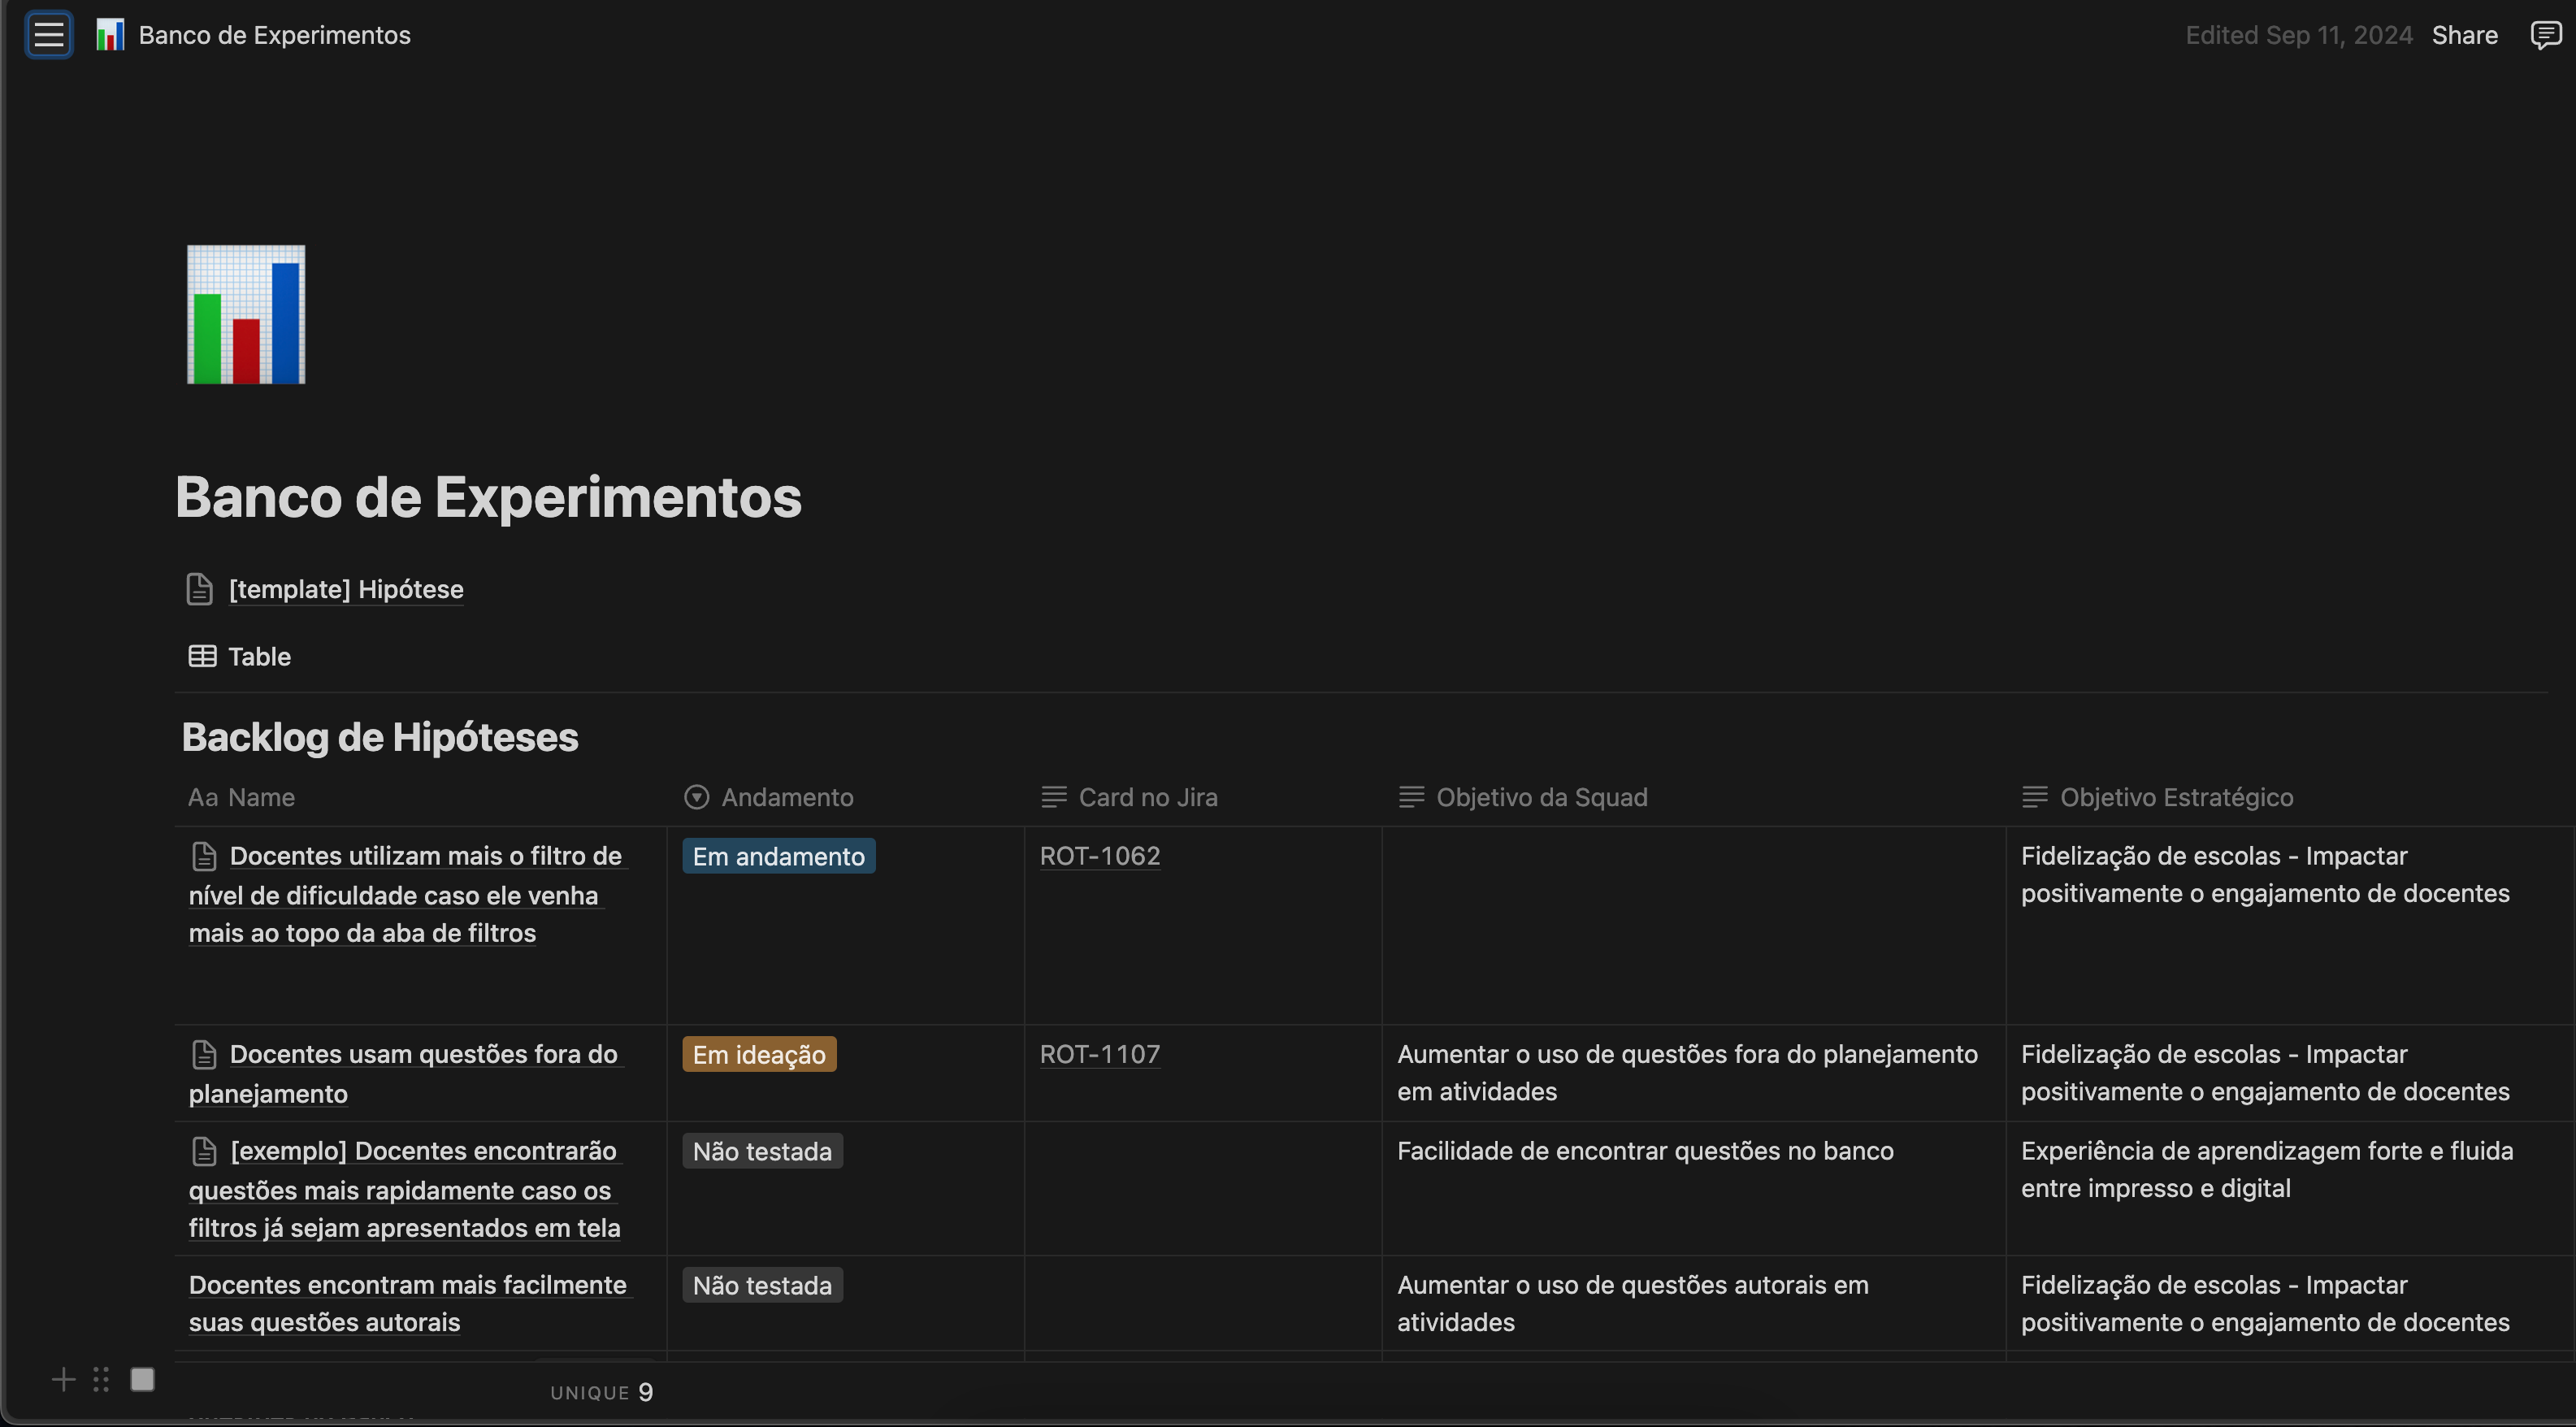
\includegraphics[width=1\linewidth]{figuras/notion_backlog.png}
        \begin{center}
            \text{Fonte: Autor}
        \end{center}
        \label{fig:notion-backlog}
    \end{figure}
    
    
    
    \begin{figure}
        \centering
        \caption{Página de Hipótese Individual no Notion}
        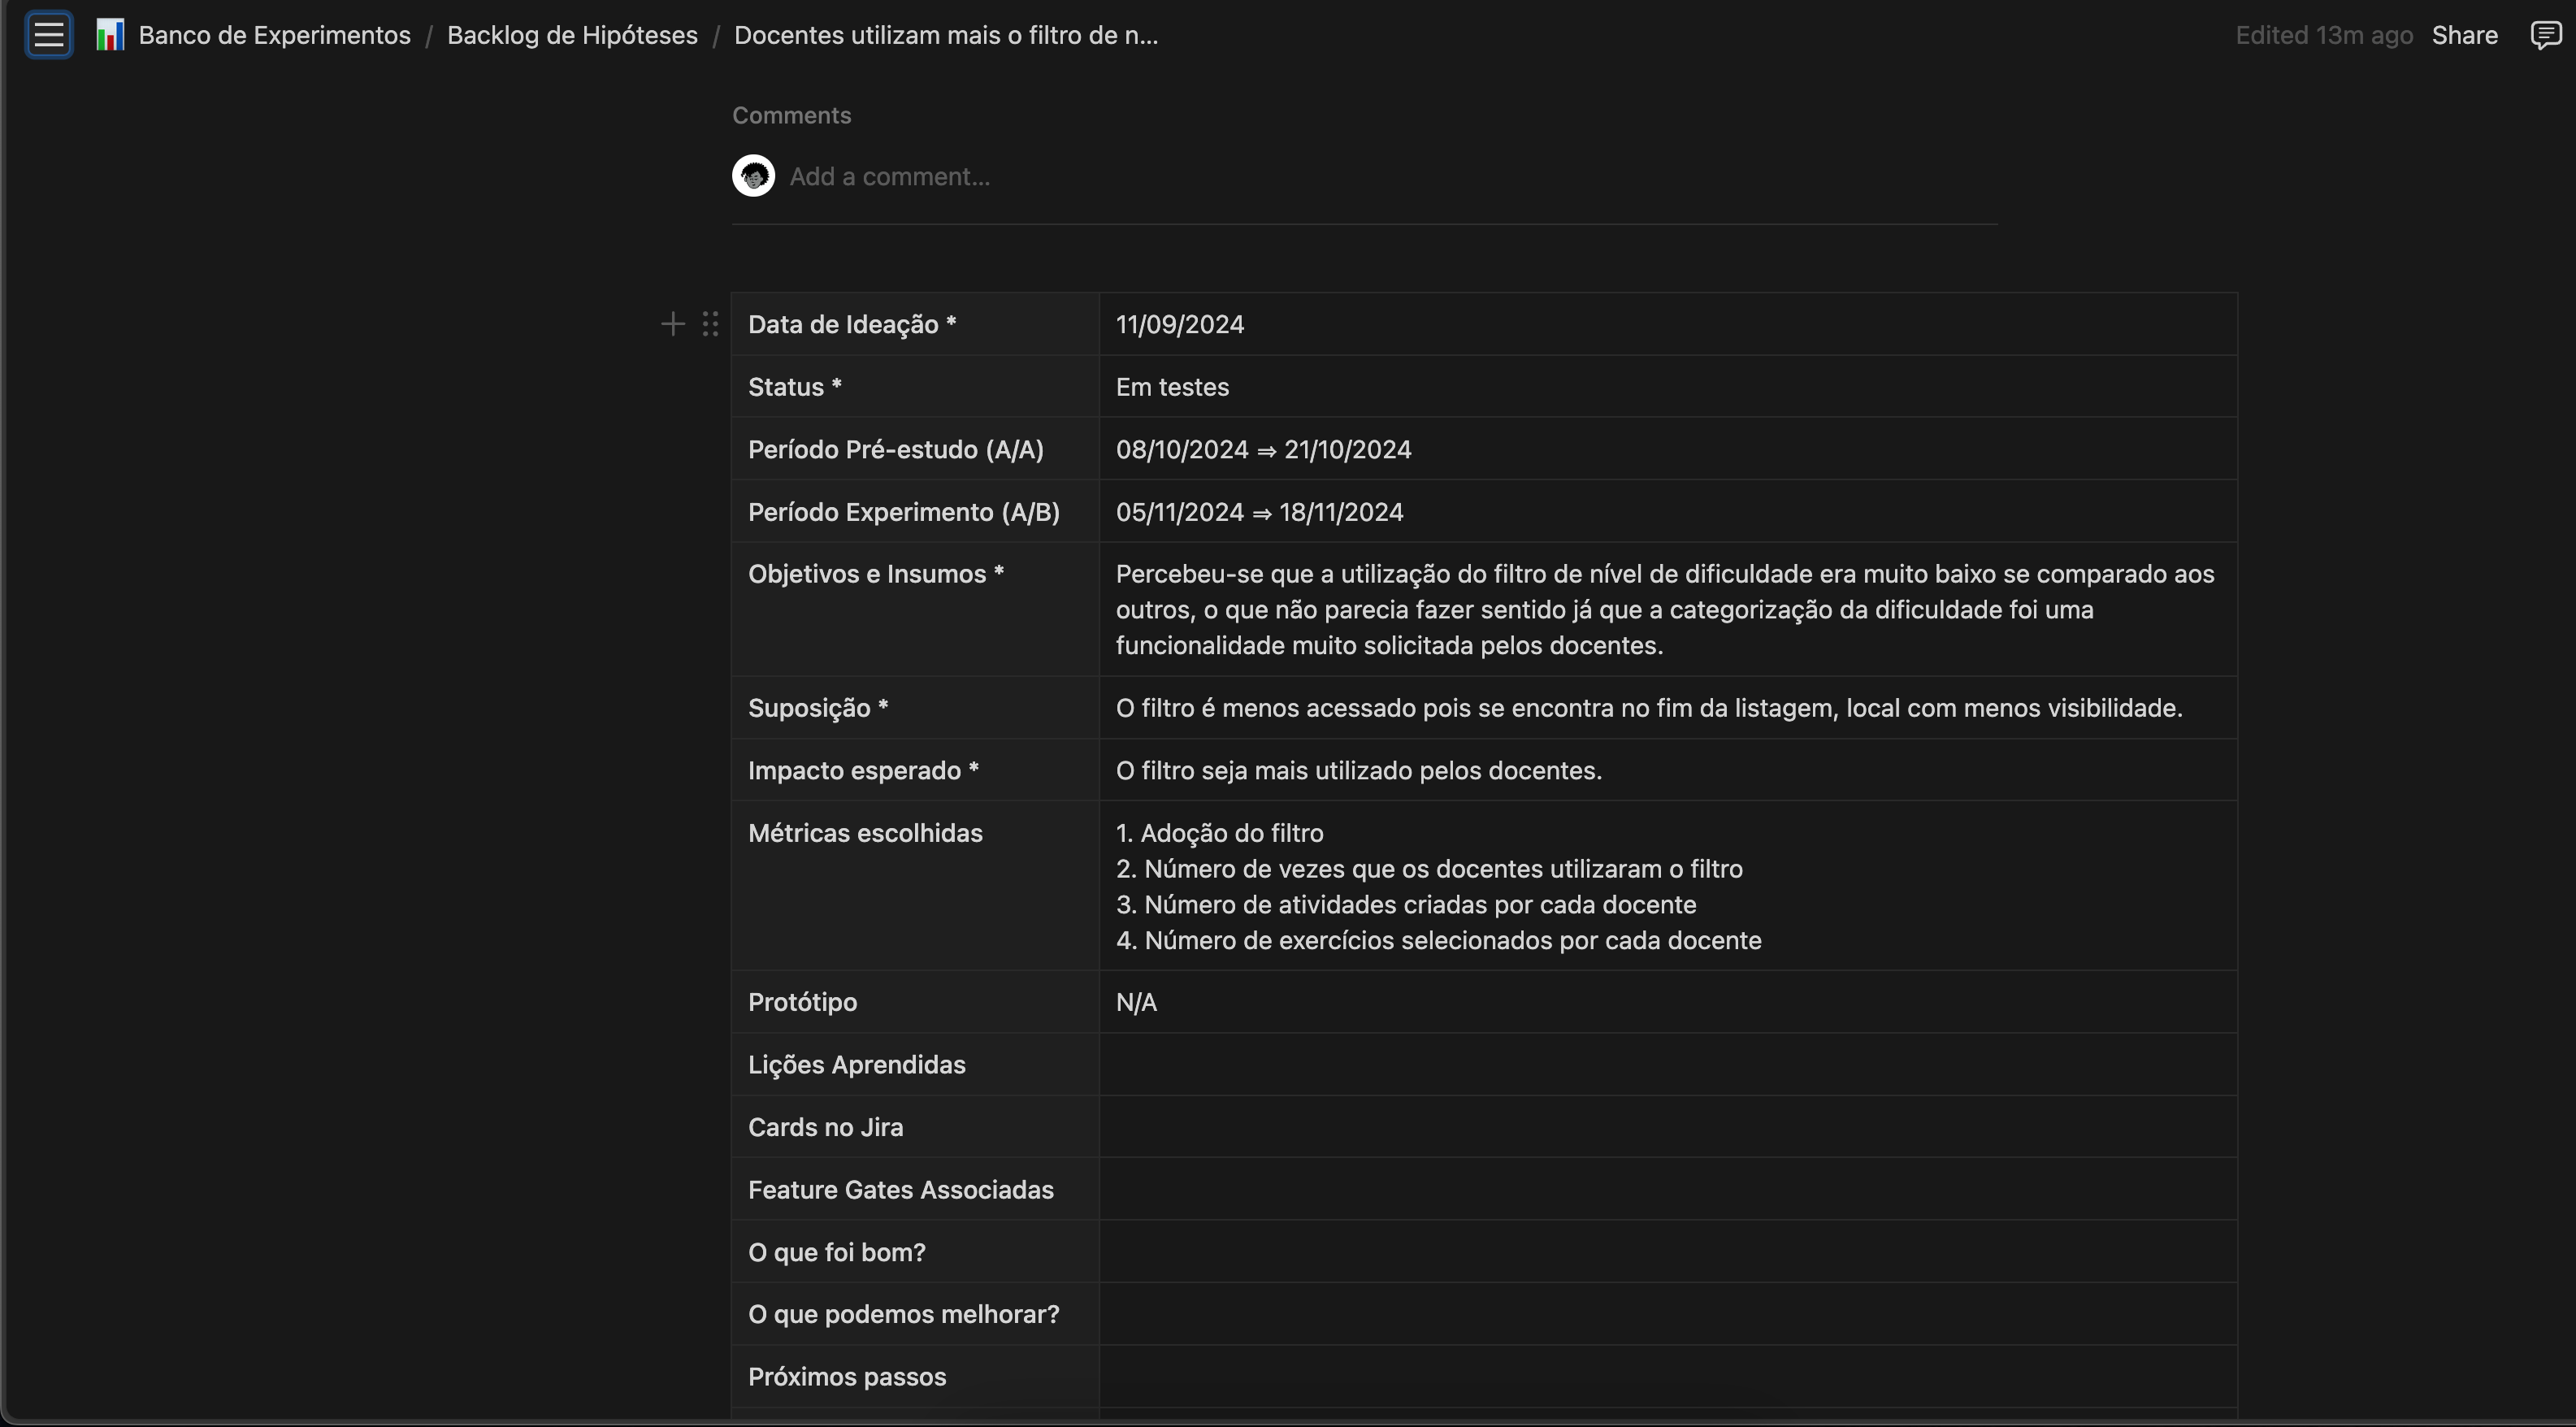
\includegraphics[width=1\linewidth]{figuras/notion_hipotese.png}
        \begin{center}
            \text{Fonte: Autor}
        \end{center}
        \label{fig:notion-hipotese}
    \end{figure}